% Packages

\documentclass{beamer}
\setcounter{tocdepth}{1}
\usepackage{graphicx}
\usepackage[export]{adjustbox}
\graphicspath{{Images/}{./}} % Specifies where to look for included images (trailing slash required)
\usepackage{tikz}
\usepackage{gensymb}
\usepackage{booktabs} % Allows the use of \toprule, \midrule and \bottomrule for better rules in tables
\usepackage{pgfplots}
\usepackage{tikz}
\pgfplotsset{width=6cm, compat=newest, every tick label/.append style={scale=0.5}}

% Command
\newcommand{\blank}{\begin{frame}
\end{frame}}


% Theme
\usetheme{Madrid}

% Font
\usefonttheme{serif}
\usepackage{newtxtext,newtxmath}
\usepackage[default]{lato}

% Inner theme
\useinnertheme{circles}

% Information
\title{Review: Coordinate geometry}
\author{Kin Hei Wong}
\date{\today}
%%%%%%%%%%%%%%%%%%%%%%%%%%%%%%%%%%%%%%%%%%%%%%%%%%%%%%%%%%
\begin{document}

% Title slide
\begin{frame}
    \titlepage
\end{frame}

% Table of Content
\begin{frame}
    \frametitle{Presentation overview}
    \tableofcontents
\end{frame}
%%%%%%%%%%%%%%%%%%%%%%%%%%%%%%%%%%%%%%%%%%%%%%%%%%%%%%%%%%%
% Body slides

\section{2A - Distance and midpoints}
\begin{frame}
    \frametitle{2A}
    \begin{center}
        \title{Distance and midpoints}
        \maketitle
    \end{center}
\end{frame}

\begin{frame}[t]
    \frametitle{Midpoint of line}
    We always find the midpoint between two coordinates by the formula:\\
    \begin{block}{Midpoint of line segment}
        $(\frac{x_1 + x_2}{2}, \frac{y_1 + y_2}{2})$
    \end{block}
    \begin{block}{Example 1}
        Find the midpoint of the line segment joining A(2,6) with B(-3,-4).
    \end{block}
\end{frame}

\begin{frame}[t]
    \frametitle{Distance - Here comes Pythagoras' theorem}
    Of course, Phythagoras' theorem always comes in handy.
    \begin{block}{Distance between two coordinates}
        Let $A = (x_1, y_1)$ and $B = (x_2, y_2)$\\
        $AB = \sqrt{(x_2 - x_1)^2 + (y_2 - y_1)^2}$
    \end{block}
    \begin{block}{Example 2}
        Calculate the distance EF if E is (-3,2) and F is (4,2).
    \end{block}
\end{frame}

\begin{frame}
    \frametitle{Exercise 2A}
\end{frame}
%%%%%%%%%%%%%%%%%%%%%%%%%%%%%%%%%%%%%%%%%%%%%%%%%%%%%%%%%%%

\section{2B - The gradient of a straight line}
\begin{frame}
    \frametitle{2B}
    \begin{center}
        \title{The gradient of a straight line}
        \maketitle
    \end{center}
\end{frame}

\begin{frame}[t]
    \frametitle{Gradient = rise over run}
    \begin{block}{Gradient}
        Gradient $m = \frac{rise}{run} = \frac{y_2-y_1}{x_2 - x_1}$
    \end{block}
    \begin{block}{Example 3}
        \begin{center}
            
\includegraphics[width = 8cm]{Example3.png}
        \end{center}        
    \end{block}
\end{frame}

\begin{frame}[t]
    \frametitle{More examples}
    \begin{block}{Example 4}
        Find the gradient of the line that passes through the points (1,6) and (-3,7).
    \end{block}
\end{frame}

\begin{frame}
    \frametitle{Tangent of an angle of slope}
    We know:\\
    \begin{center}
        $tan(\theta) = \frac{\text{opposite}}{\text{adjacent}}$
    \end{center}
    Then, we can apply it to coordinates too!
    \begin{block}{Tangent with coordinates}
        $m = \pm\frac{y_2-y_1}{x_2 - x_1}$\\
        $m = \pm tan(\theta)$
    \end{block}
    Exercise: What is the restriction to coordinates $x_2$ and $x_1$.
\end{frame}

\begin{frame}[t]
    \frametitle{Examples marching in}
    \begin{block}{Example 5}
        Determine the gradient of the line passing through the points (3,2) and (5,7) and the angle that the line makes with the positive direction of the x-axis.
    \end{block}
    \begin{block}{Example 6}
        Determine the gradient of the line passing through the points (5, 3) and (-1,5) and the
        angle that the line makes with the positive direction of the x-axis.
    \end{block}
\end{frame}
\blank

\begin{frame}
    \frametitle{Prove of negative gradient}
\end{frame}

\begin{frame}
    \frametitle{Exercise 2B}
\end{frame}
%%%%%%%%%%%%%%%%%%%%%%%%%%%%%%%%%%%%%%%%%%%%%%%%%%%%%%%%%%%

\section{2C - The equation of a straight line}
\begin{frame}
    \frametitle{2C}
    \begin{center}
        \title{The equation of a straight line}
        \maketitle
    \end{center}
\end{frame}

\begin{frame}
    \frametitle{$y = mx + c$}
    It is actually relatively easy to understand what $y = mx + c$ is:
    \begin{block}{Equation}
        $x, y$ = $(x,y)$ coordinates\\
        $c$ = y-axis intercept\\
        $m$ = gradient we leartn previously
    \end{block}
    When the question ask to find the equation, then we just find the value of $m$ and $c$.\\
    Leave the answer as: $y = mx + c$ (E.g. $y = 4x + 5$)
\end{frame}

\begin{frame}
    \frametitle{Why is equation so important?}
    Equation shows the relation between two things with some factors with them (which are $m$ and $c$).\\
    Suppose we rent a car from GoGet (no they did not sponsor me), Let $c$ be the fixed cost of renting a car, $m$ be the charge for each hour, $x$ be the number of hours, $y$ be the total charge\\
    Try compute it in desmos!\\
    \url{https://www.desmos.com/}
\end{frame}

\begin{frame}[t]
    \frametitle{Examples}
    \begin{block}{Example 7}
        Find the gradient and y-axis intercept of the line y = 3x-4.
    \end{block}
    \begin{block}{Example 8}
        Find the equation of the line with gradient -3 and y-axis intercept 5.
    \end{block}
    \begin{block}{Example 9}
        State the gradient and y-axis intercept of the line 3y + 6x = 9.
    \end{block}
\end{frame}
\begin{frame}
\end{frame}

\begin{frame}
    \frametitle{Where're the coordinates?}
    Suppose you are living at a coordinate $(x_0, y_0)$ (and you know this coordinate). You want to go to your friend's house at $(x,y)$. You do not know specifically what the coordinates are 
    but you know what speed you were going approximately, and we let this speed be m. (Given that you only walk straight, you know the distance and time [I know, I know, a lot of assumptions]).\\
    We can actually calculate what you friend's house coordinate is at!
    \begin{block}{Point-gradient form}
        $y-y_0 = m(x-x_0)$\\
        Exercise: Does this equation look familiar to you?
    \end{block}
\end{frame}

\begin{frame}
    \frametitle{Examples!}
    \begin{block}{Example 10}
        Find the equation of the line which passes through the point (-1,3) and has gradient 4.
    \end{block}
    \begin{block}{Example 11}
        Find the equation of the line that passes through the point (3,2) and has a gradient of -2.
    \end{block}
\end{frame}
\begin{frame}
\end{frame}

\begin{frame}[t]
    \frametitle{What if two points are given only?}
    If two points are given, we can find the gradient!\\
    Exercise: How? (Hint: Look back at the equations we learnt)
    Then, after finding the gradient, we just put it in equation form by taking one of the equation into point-gradient form!\\
    \begin{block}{Example 12}
        Find the equation of the straight line passing through the points (1,-2) and (3,2).
    \end{block}
\end{frame}

\begin{frame}[t]
    \frametitle{Example... again...}
    \begin{block}{Example 13}
        Find the equation of the straight line with y-axis intercept -3 which passes through the
        point with coordinates (1,10).
    \end{block}
\end{frame}

\begin{frame}
    \frametitle{Two different intercepts - I swear the textbook is just giving different cases}
    We can derive the equation from gradient formula into:\\
    \begin{block}{Intercept form}
        Two intercepts are: $(a,0), (0,b)$
        $\frac{x}{a} + \frac{y}{b} = 1$
        where:\\
        $a$ = $x$-intercept\\
        $b$ = $y$-intercept
    \end{block}
\end{frame}

\begin{frame}[t]
    \frametitle{Last... example...... in this part}
    \begin{center}
        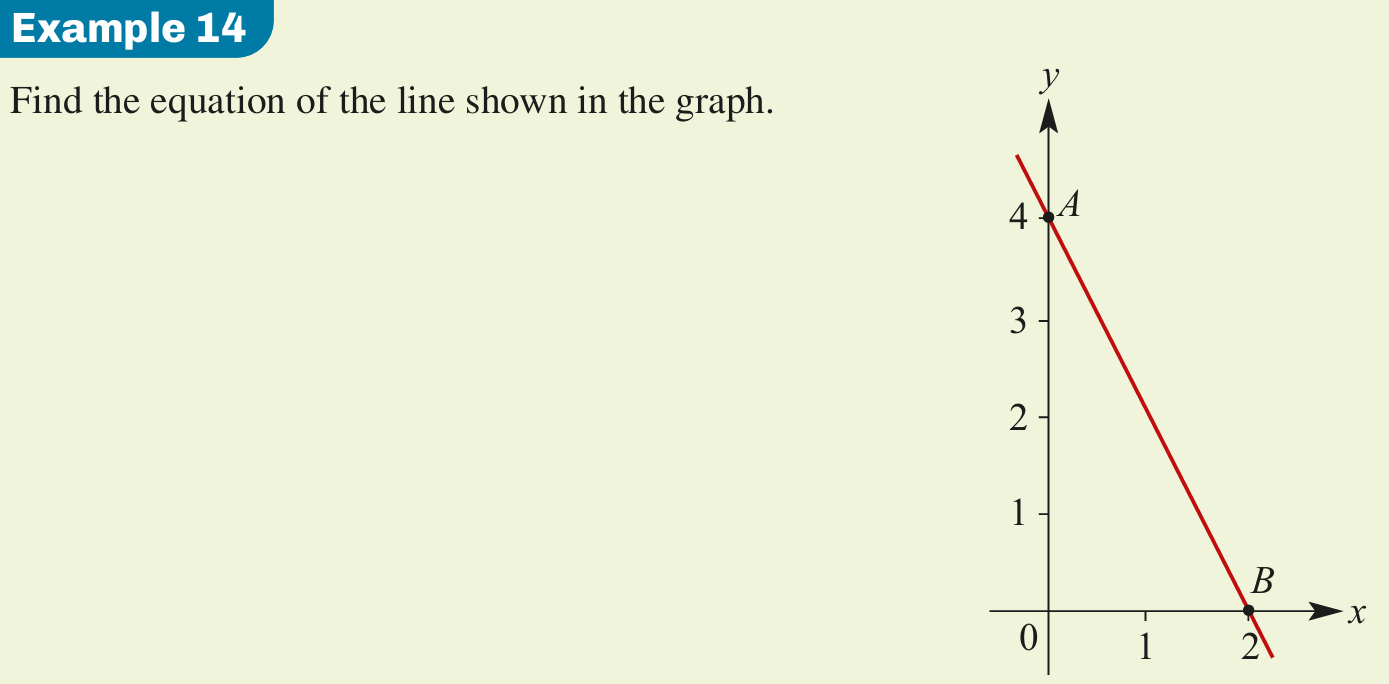
\includegraphics[width = 10cm]{Ex14.png}
    \end{center}
\end{frame}
\begin{frame}
\end{frame}

\begin{frame}
    \frametitle{Exercise 2C}
    \begin{center}
        
\includegraphics[width = 5cm]{Wait.jpg}
    \end{center}
\end{frame}
%%%%%%%%%%%%%%%%%%%%%%%%%%%%%%%%%%%%%%%%%%%%%%%%%%%%%%%%%%%

\section{2D - Graphing straight lines}
\begin{frame}
    \frametitle{2D}
    \begin{center}
        \title{Graphing straight lines}
        \maketitle
    \end{center}
\end{frame}

\begin{frame}[t]
    \frametitle{Sketching time!}
    Before we start: (Sketch vs draw)\\
    Sketch: Coordinates at axis, shape of graph, turning point (some questions only)\\
    Draw: Find all x and y value requested\\
    \begin{block}{Example 15 and 16}
        \begin{enumerate}
            \item Sketch the graph $2x + 4y = 10$
            \item Sketch the graph $y = 2x-6$
        \end{enumerate}
    \end{block}
\end{frame}

\begin{frame}
\end{frame}

\begin{frame}[t]
    \frametitle{Angle of the slope}
    \begin{block}{Example 17}
        For each of the following lines, find the magnitude of the angle $\theta$ (2.d.p.) that the line makes with the positive direction of the $x$-axis:\\
        \begin{enumerate}
            \item $y = 2x+3$
            \item $3y = 3x-6$
            \item $y = -0.3x + 1.5$
        \end{enumerate}
    \end{block}
\end{frame}
\blank

\begin{frame}
    \frametitle{Exercise 2D}
\end{frame}
%%%%%%%%%%%%%%%%%%%%%%%%%%%%%%%%%%%%%%%%%%%%%%%%%%%%%%%%%%%

\section{2E - Parallel and perpendicular lines}
\begin{frame}
    \frametitle{2E}
    \begin{center}
        \title{Parallel and perpendicular lines}
        \maketitle
    \end{center}
\end{frame}

\begin{frame}
    \frametitle{Parallel vs perpendicular lines}
    Parallel: same $m, \theta$, others can be different
    Perpendicular: \\
    Given two straight line equations:$y = m_1x + c_1$ and $y = m_2x + c_2$\\
    IF $m_1m_2 = -1$, then both the equations are perpendicular to each other.\\
    Also: $\theta$ = $90 \degree$
\end{frame}

\begin{frame}[t]
    \frametitle{Examples}
    \begin{block}{Example 18}
        Find the equation of the straight line which passes through (1,2) and is:\\
        \begin{enumerate}
            \item parallel to the line with equation $2x - y = 4$
            \item perpendicular to the line with equation $2x - y = 4$.
        \end{enumerate}
    \end{block}
\end{frame}

\begin{frame}[t]
    \frametitle{Another one}
    \begin{block}{Example 19}
        The coordinates of the vertices of a triangle ABC are A(0,-1), B(2,3) and C(3,-2$\frac{1}{2}$)
        Show that the side AB is perpendicular to the side AC.
    \end{block}
\end{frame}
\blank

\begin{frame}
    \frametitle{Exercise 2E}
\end{frame}
%%%%%%%%%%%%%%%%%%%%%%%%%%%%%%%%%%%%%%%%%%%%%%%%%%%%%%%%%%%

\section{2F - Families of straight line}
\begin{frame}
    \frametitle{2F}
    \begin{center}
        \title{Families of straight line}
        \maketitle
    \end{center}
\end{frame}

\begin{frame}
    \frametitle{WE ARE FAMILY}
    As long as we have one parameter (not variables), then it has a family.\\
    E.g.\\
    $y=mx$\\
    $y = 3x + c$\\
    $y = mx + 2$
\end{frame}

\begin{frame}
    \frametitle{Examples}
    \begin{block}{Example 20}
        Find the value of $m$ if the line $y = mx + 2$ passes through the point (3,11).
    \end{block}
    \begin{block}{Example 21}
        A family of lines have equations of the form $y = mx + 2$, where m is a negative number.
        \begin{enumerate}
            \item  Find the $x$-axis intercept of a line in this family in terms of $m$.
            \item For which values of $m$ is the $x$-axis intercept greater than 3?
            \item  Find the equation of the line perpendicular to the line $y = mx + 2$ at the point (0,2)
        \end{enumerate}
    \end{block}
\end{frame}

\begin{frame}
    \frametitle{Exercise 2F}
\end{frame}
%%%%%%%%%%%%%%%%%%%%%%%%%%%%%%%%%%%%%%%%%%%%%%%%%%%%%%%%%%%

\section{2G - Linear models}
\begin{frame}
    \frametitle{2G}
    \begin{center}
        \title{Linear models}
        \maketitle
    \end{center}
\end{frame}

\begin{frame}[t]
    \frametitle{Finally, some real-life applications}
    \begin{block}{Example 22}
        A historical site charges a tour company for priority entrance to the site. The charge
        consists of a monthly fee of $\$200$ plus $\$3.50$ for each tourist brought to the site. Construct
        a cost function that describes the monthly charge and sketch the linear graph for this.
    \end{block}
\end{frame}

\begin{frame}[t]
    \frametitle{Another one}
    \begin{block}{Example 23}
        A car starts from point A on a highway $10km$ past the Wangaratta post office. The car travels at a constant speed of $90km/h$ 
        towards picnic stop B, which is $120km$ further on from A. Let $t$ hours be the time after the car leaves point A.\\
        \begin{enumerate}
            \item Find an expression for the distance $d_1$ of the car from the post office at time $t$ hours.
            \item Find an expression for the distance $d_2$ of the car from point B at the time $t$ hours.
            \item On seperate sets of axes, sketch the graphs of $d_1$ against $t$ and $d_2$ against $t$ and state the gradient of each graph.
        \end{enumerate}
    \end{block}
\end{frame}

\begin{frame}
    \frametitle{Exercise 2G}
\end{frame}
%%%%%%%%%%%%%%%%%%%%%%%%%%%%%%%%%%%%%%%%%%%%%%%%%%%%%%%%%%%

\section{2H - Simultaneous linear equations}
\begin{frame}
    \frametitle{2H}
    \begin{center}
        \title{Simultaneous linear equations}
        \maketitle
    \end{center}
\end{frame}

\begin{frame}
    \frametitle{Geometry of simultaneous equations}
    If unique solution: only one point being intersecting\\
    If $\infty$ solutions: they are lines being coincide\\
    If no solution: lines are parallel
\end{frame}


\begin{frame}[t]
    \frametitle{Describe it}
    \begin{block}{Example 24}
        Explain why the simultaneous equations $2x + 3y = 6$ and $4x + 6y = 24$ have no solution. 
    \end{block}
    \begin{block}{Example 25}
        The simultaneous equations $2x + 3y = 6$ and $4x + 6y = 12$ have infinitely many solutions.
 Describe these solutions through the use of a parameter.
    \end{block}
\end{frame}

\begin{frame}[t]
    \frametitle{More problems}
    \begin{block}{Example 26}
        The family of lines $y = mx + 2$ with varying gradient $m$ all pass through the point (0,2).\\
        \begin{enumerate}
            \item  For what values of $m$ does the line $y = mx +2$ not intersect the line $y = 5x- 3$?
            \item For what values of $m$ does the line $y = mx +2$ intersect the line $y = 5x- 3$?
            \item  If the line $y = mx+2$ intersects the line $y = 5x - 3$ at the point (5,22), find the value
            of $m$.
        \end{enumerate}
    \end{block}
\end{frame}

\begin{frame}[t]
    \frametitle{Bruh... why so many problems}
    \begin{block}{Example 27}
        The lines $y = x +k$ and y = mx+4intersect at (1,3). Find the values of $m$ and $k$.
    \end{block}
    \begin{block}{Example 28}
        The lines $(m-2)x+y = 2$ and $mx+2y = k$ intersect at (2,8). Find the values of $m$ and $k$.
    \end{block}
\end{frame}

\begin{frame}[t]
    \frametitle{Are you done yet?}
    \begin{block}{Example 29}
        Consider the simultaneous linear equations $(m-2)x + y = 2$ and $mx + 2y = k$. Find the
        values of $m$ and $k$ such that the system of equations has:\\
        \begin{enumerate}
            \item no solution
            \item infinitely many solutions
            \item a unique solution
        \end{enumerate}    
    \end{block}
\end{frame}

\begin{frame}[t]
    \frametitle{Application... really?}
    \begin{block}{Example 30}
        There are two possible methods for paying gas bills:\\
    Method A: A fixed charge of $\$25$ per quarter + 50c per unit of gas used\\
    Method B: A fixed charge of $\$50$ per quarter + 25c per unit of gas used\\
    Determine the number of units which must be used before method B becomes cheaper than method A.
    \end{block}
\end{frame}

\begin{frame}[t]
    \frametitle{Example 31}
    Robyn and Cheryl race over 100 metres. Robyn runs so that it takes $a$ seconds to run
    1 metre, and Cheryl runs so that it takes $b$ seconds to run 1 metre. Cheryl wins the race by
    1 second. The next day they again race over 100 metres but Cheryl gives Robyn a 5-metre
    start so that Robyn runs 95 metres. Cheryl wins this race by 0.4 seconds. Find the values
    of $a$ and $b$ and the speed at which Robyn runs.
\end{frame}
\blank

\begin{frame}
    \frametitle{Exercise 2H}
\end{frame}

\end{document}